\documentclass{llncs}
\usepackage{makeidx}  % allows for indexgeneration
\usepackage[pdftex]{graphicx} % PNGs
\usepackage{amsmath, amssymb} % algebra
%\usepackage[ngerman]{babel}
\usepackage[utf8x]{inputenc}
\usepackage[T1]{fontenc} 
\usepackage[procnames]{listings} % for sourcecode
\usepackage{graphviz} % graphs
\usepackage{array,multirow} % tables
\usepackage{afterpage} % figures
\usepackage{float} % figures

\lstset{%
  	%language=Java,
	basicstyle=\small,
	frame=single,
	sensitive=true,
	keywordsprefix=P,
	keywords={END,W,W1},
	keywordstyle=\bfseries,
	identifierstyle=\ttfamily,
	procnamestyle=\bfseries,
	procnamekeys={P},
	literate={<}{$<$}1 {>}{$>$}1 {=}{$=$}1 {<=}{$\leq$}1 {>=}{$\geq$}1 {=>}{{$\Rightarrow$}}1 {->}{{$\rightarrow$}}1
	}
%\renewcommand{\textfraction}{0.05}
%\renewcommand{\topfraction}{0.95}
%\renewcommand{\bottomfraction}{0.95}
%\setcounter{totalnumber}{5}
\restylefloat{figure}
\begin{document}
%
%\frontmatter          % for the preliminaries
%
\pagestyle{headings}  % switches on printing of running heads
%
\mainmatter % start of the contributions
%
\title{The Plankalkül}
\subtitle{An Early High-Level Programming Language}
%
\titlerunning{The Plankalkül}  % abbreviated title (for running head)
%                                     also used for the TOC unless
%                                     \toctitle is used
%
\author{Tim Felgentreff}
\date{\today}
%
\authorrunning{Tim Felgentreff}   % abbreviated author list (for running head)
%
%%%% modified list of authors for the TOC (add the affiliations)
\tocauthor{Tim Felgentreff (Hasso-Plattner-Institute)}
%
\institute{History of Programming Languages, Software Architecture Group, Hasso-Plattner-Institut, Universität Potsdam, D-14482 Potsdam, Germany,\\
\email{tim.felgentreff@student.hpi.uni-potsdam.de}}

\maketitle
\begin{abstract}
   Lectures on the history of computing have for a long time 
   ignored any development on the matter before the end of World War II. 
   This for a long time supported the view that the roots of 
   computing and programming languages lie with large corporations 
   like IBM and the Universities.
   Although today
   the German engineer Konrad Zuse is widely recognised
   as the first inventor of general purpose computing machines, 
   and his automatons are widely explored, another invention of 
   his, the very first concept of a 
   high-level programming language, has remained largely unheard of.
   This paper explores Zuse's language, ``Der Plankalkül'', 
   and describes some its background and concepts, as well as its 
   meaning for the history of programming languages.
\end{abstract}
 \section{Introduction}
   Every one who works with computers on a professional level has 
   at some time heard of Konrad Zuse and his Z3, the first fully 
   automatic programmable computer. This computer, built in the 
   house of his parents, from old phone relais, by a man who has had no 
   previous contact with other scientists working on automatic computation, 
   has been so thoroughly reviewed and been written about, that it 
   stands synonym for Konrad Zuse's life work.

   However, parallel to his efforts on building the Z1 through Z3, Zuse
   also worked on his programming language, which he called ``Plan Calculus''
   to show its sources in the ``logical caclulus''. The first notes about
   this language appeared in his notebooks in May, 1939~\cite{rojas2002konrad}. The \emph{Genesis}
   of the Plankalkül lies in the years 1942 to 45.

   In this paper we will elaborate on the historical background in which 
   Zuse conducted his work, as well as explore earlier and parallel attempts 
   at similar work. After exploring Zuse's incentive for creating a programming 
   language, we will present his Plan Calculus in more detail, giving an overview 
   of its syntax and data-structures as well as its higher-level constructs and compare 
   those to modern programming languages. Finally, we consider the impact Zuse
   had with his language on the popular programming languages which came after.
 \section{History}
   Work on mechanical calculation goes back to the invention of the Abacus, but one 
   of the first notable ``computing'' machines was Charles Babbage's \emph{Analytical Engine},
   which he first described in 1837. It was for this theoretical machine (which was not built until the 
   late 1960's), that Ada Lovelace later wrote an instruction set for calculating the Bernoulli numbers.
   These instructions, written in an assembler-like language, are today considered the very first computer program.

   Due to lack of interest and money, the \emph{Engine} was never built and the next 
   time somebody should concern himself with computation in such depth was 
   one hundred years later. During the 1930's, one Alan Turing started his work on computable numbers
   and Konrad Zuse began working on his Z1.
 \subsection{Zuse and Computing}
   Konrad Zuse was a civil engineer in the Germany of the 1920's. He became annoyed by
   the repetitive nature of the computations he had to perform at his workplace and began to 
   to consider building machines to perform such dull computations.
   Due to his engineering background he had never come in contact with previous 
   ideas of the kind and the political developments at the time kept him 
   from exploring parallel developments in the United States at the time.

   To work on his first machine, the V1 (later renamed to Z1, not to be 
   confused with the V-line of German rockets), Zuse borrowed money
   from friends and relatives. He built the Z1 at his parents home, cutting the 
   pieces he needed with a jigsaw. We know today that his design would have worked,
   but the rough nature of the parts the computer was built of made it extremely unreliable,
   and so Zuse notes in May, 1939: ``Rechenwerk fertig, aber funktioniert schlecht''\cite{rojas2002plankalkuel}.
 \subsection{The Z1 to Z4}
   Working almost completely on his own, Zuse designed and built machines 
   which had many characteristics of today's computers. All his machines
   had binary floating-point arithmetics, separate \emph{Arithmetic logic units} (ALU), 
   a central processor and general purpose memory banks.
   Programs were written on punched tape and his Z1 and Z3 had 24bit word-sizes
   and arithmetic exception handling. A scheme if the Z1 can be seen in Fig.\ref{fig:z1}.
   
  \begin{figure}[t]
    \centering
    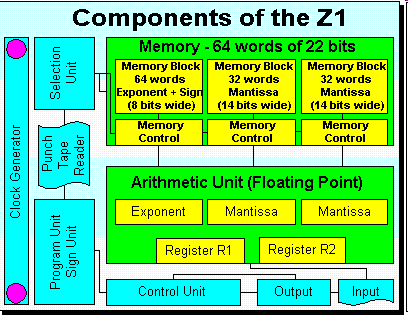
\includegraphics[width=0.5\linewidth]{img/z1.png}
    \caption{Top-down view of the Z1\cite{epegmagHorstzuse}}
    \label{fig:z1}
  \end{figure}

   Zuse basically created the von Neumann architecture (without saving the program to memory)
   before it was even formulated\cite{epegmagHorstzuse} 
   and invented a notation which he called ``combinatorics of conditionals'' which was
   identical to the propositional calculus, as Zuse himself realized later.
 \subsection{The Vision of a Chess Game}
   Zuse knew the potential of his machine. He told his co-workers and 
   friends, that one day, he would teach it to play a game of chess 
   against him. However, on trying to create an implementation, he realized 
   that ``even simple relations are very difficult to express''.
   
   Zuse concerned himself with concepts of boolean algebra and found many 
   of his ideas reflected in it. He derived, that any concept were expressible
   using only the basic operations NOT, AND and OR. He developed this epiphany 
   to conceptually create a \emph{logic machine} (Fig. \ref{fig:logicmachine}). 
   
   Konrad Zuse intuitively 
   understood that from simple building blocks, as were his logic machines, 
   he could create hierarchical structures that would be able to solve any 
   computationally solvable problem (although, in his notes he never concerns 
   himself with the question of computability. He considered the chess game his 
   ultimate test for the capabilities of his machines).
 \section{The Plankalkül}
    - implicit to explicit
    - automatic mapping
 \subsection{Motivation}
  \begin{figure}[bt]
    \centering
    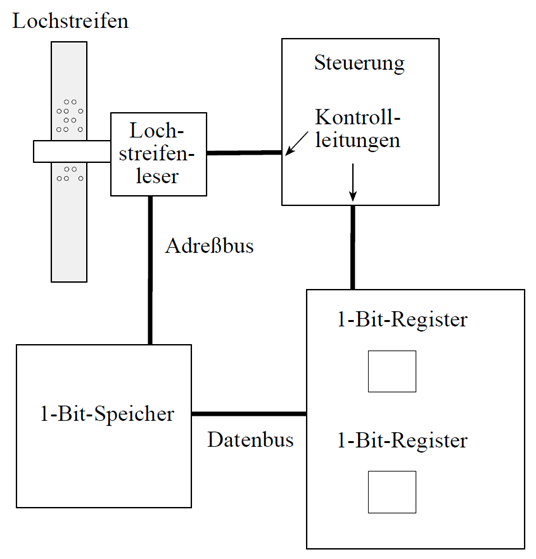
\includegraphics[width=0.4\linewidth]{img/logicmachine.png}
    \caption{A scheme of Zuse's \emph{logic machine}\cite{rojas2002plankalkuel}}
    \label{fig:logicmachine}
  \end{figure}

   Zuse had realized early on, through his study of propositional logic, that any 
   logical statement could be mapped onto his logistic machine. He understood that
   having a high level way of programming \dots\\
    - high level programming, low level execution\\
    - re-usable components (Programmpläne)
 \subsection{Basic Concepts}
   In the following we would like to present some of 
   the concepts which can be found in the Plankalkül 
   and provide reasons for them, were they seem far-fetched 
   or surprising.
   
   When considering Konrad Zuse's language, we have to keep 
   in mind his hardware development background. While Zuse strived 
   to create a universial language that made it easy to write 
   programs for his computers, he eventually meant for them to
   be converted into basic statements to run on hierarchies of 
   his logistic machines.
   
   From the start, Zuse realized that all computation can be expressed 
   in the form $F(x) \Rightarrow R$. he considered computing in a very 
   general sense, writing in his notes: ``Rechnen heißt: Aus
   gegebenen Angaben nach einer Vorschrift neue Angaben bilden''\cite{bauer1972plankalkuel}

   Additionally, Zuse decided to use the binary 
   true/false logic as most basic type. While many modern languages still 
   do not have a bit type (e.g. C, C++), use of the binary system as such 
   for algebra was not even widely explored at the time. As late as 1938 Bell Labs created a 
   research program for the matter, something Zuse did not know of. The first 
   language after the Plankalkül to implement a binary data type for use in 
   boolean logic was ALGOL 60.
   
   Those basic ideas, while noteworthy, do not make the language any more
   high-level than the weaving descriptions of one Ada Lovelace. 
   Zuse intended his language to have a much stronger expressibility. 
   Especially in hindsight it is remarkable 
   to what extend Zuse already considered standard features of modern 
   programming languages for his Plan Calculus.
   
   \begin{description}
     \item[GOTO] Der Plankalkül does not have 
       a GOTO statement. While this may be due to some excellent
       foresight of Zuse's, the GOTO statement would also be
       difficult to implement with punched tape.
     \item[Recursion] There is no recursion.
       This is due to the \emph{call-by-value} nature of the 
       language. One would have to use a fixed point combinator
       in order to express recursive statements. The 
       ideas of Zuse's hierarchically structured machines would not 
       allow implementation of such behavior.
     \item[Loops] The Plan Calculus has a powerful loop statement, 
       that can be used either like a modern limited loop (for .. to) 
       or a conditional loop (while). This made the language Turing
       complete even though Zuse did not know the term nor the 
       concept at the time.
     \item[Branches] Conditional branching was already implemented 
       in the Z3 and the concept was included in his calculus, too.
     \item[Algebraic Notation] Konrad Zuse derived his program 
       notation from the propositional calculus which makes
       it more natural to read for the programmer than assembler like 
       language.
   \end{description}
   These concepts give reasons for considering Der Plankalkül a
   high-level programming language. They are explained in more detail 
   in the following sections.
 \subsection{Notation}
 \begin{figure}[tb]
   \begin{center}
     \begin{tabular}[bt]{c c c c c c c | c}
       V & + & V & $\Rightarrow$ & Z & {\LARGE\multirow{3}{*}{$\swarrow$}} & Z & ~\\
       0 &   & 1 &               & 1 &   & 0 & {\bf V}\\
       1 &   &   &               &   & &   & {\bf K}\\
       2.0 & & 2.0 &             & 2.0 & & 0 & {\bf S} \\
       \multicolumn{3}{c}{$\underbrace{\qquad\qquad}_{\text{Addition}}$}
       	& & \multicolumn{3}{c}{$\underbrace{\qquad\qquad\quad}_{\text{Dynamic select}}$} \\
	\multicolumn{7}{c}{$\underbrace{\qquad\qquad\qquad\qquad}_{\text{Assignment}}$} &
     \end{tabular}
   \end{center}
   \caption{The Tabular Notation of the Plan Calculus}
   \label{fig:notation}
 \end{figure}
   Certainly one of the most obvious deviations from almost all other programming 
   languages is the tabular notation Zuse chose to write his ``Program Plans'' in\ref{fig:notation}. 
   
   Almost all programming languages that came afterwards were designed with the input
   methods already thought out. Zuse approached his language without being preoccupied 
   with common input methods simply for the reason that there were none. So he chose 
   to represent programs in the Plan Calculus in statements consisting of four lines. 
   The main line includes the statement essentially in its mathematical form, 
   e.g. operations, conditions or variable assignments.
   The second line, which Zuse called the \emph{Variable Line}, is used to identify 
   the variable by a subindex. The S-line, called \emph{Structure Line}, denotes the 
   structure inside the variable which determines its \emph{type}. In the example above, the variables 
   $\begin{matrix}V\\0\end{matrix}$, $\begin{matrix}V\\1\end{matrix}$ and 
   $\begin{matrix}Z\\1\end{matrix}$ are of type 2.0, and the variable $\begin{matrix}Z\\0\end{matrix}$
   has the simple type 0. In Zuse's examples the S-line is not always filled, especially when the 
   type of a variable is clear from the context, however, he notes that it simplifies understanding 
   of the formula\cite{rojas2002plankalkuel}.\\
   The K, or \emph{Component Line}, can be used to select only parts of a variables structure to operate 
   on.
 \subsection{Variables}
   -3 kinds
 \subsubsection{Types}
   Bit, \\Arrays, \\Tuples, \\Floating Point
 \subsection{Higher-level constructs}
   While, \\For-To, \\Nesting, \\If-Then, \\Blocks,
   \\multi-level-breaks
 \section{Modern implementations}
   1979, \\2000, \\2009
 \subsection{Programmatic examples}
   Bubble Sort\\
   \begin{lstlisting}
   P11 BubbleSort (V0[:20.8.0]) => R0[:20.8.0]
     N(V0[:20.8.0]) => Z0[:8.0]
     V0[:20.8.0] => Z1[:20.8.0]
     W1(Z0[:8.0]) [
       0 => Z2[:0]
       W1(Z0[:8.0]-i-2) [
         Z1[i:8.0] > Z1[(i+1):8.0] -> [
           Z1[i:8.0] => Z3[:8.0]
           Z1[i+1:8.0] => Z1[i:8.0]
           Z3[:8.0] => Z1[i+1:8.0]
           1 => Z2[:0]
         ]
       ]
       Z2[:0] = 0 -> FIN
     ]
     Z1[:20.8.0] => R0[:20.8.0]
   END
   \end{lstlisting}
     -> Run over n! times\\
     -> Break if no swap was done
     
   Insertion Sort
   \begin{verbatim}
     HUUU
   \end{verbatim}
   Chess

 
   \section{Impact on the world of programming}
   \section*{Acknowledgements}
   Thank Malte and Horst Zuse
  \bibliographystyle{splncs}
  \bibliography{kalkul}
  \clearpage
\end{document}

